\chapter{Loose-Coupled LIO}
\label{sec:loose_coupling_lio}

\section{State Variables and Problem Formulation}
\label{eq:state_and_problem_setting_loose_coupling}

In the scan matching discussed in the previous chapter, the problem was formulated as estimating only the pose $T \in {\rm SE}(3)$.
In contrast, in the LIO described in this chapter, we consider estimating the following state variables.
%
\begin{align}
  {\bf x} = \left( {}^{O}{\bf t}_{I} ~ {}^{O}R_{I} ~ {}^{O}{\bf v} ~ {\bf b}^{\omega} ~ {\bf b}^{a} \right),
  \label{eq:loose_coupling_lio_state}
\end{align}
%
where ${}^{O}{\bf t}_{I} \in \mathbb{R}^{3}$ and ${}^{O}R_{I} \in {\rm SO}(3)$ denote the translation vector and rotation matrix representing the IMU pose in the odometry frame, ${}^{O}{\bf v} \in \mathbb{R}^{3}$ denotes the velocity vector of the IMU in the odometry frame, and ${\bf b}^{\omega}, {\bf b}^{a} \in \mathbb{R}^{3}$ represent the biases of the IMU angular velocity and acceleration, respectively.
Since $\left( \log \left( R \right) \right)^{\vee} \in \mathbb{R}^{3}$, the LIO problem described in this chapter becomes one of estimating a 15-dimensional state.
It should be noted that this involves estimating the IMU pose.

Because LIO utilizes both LiDAR and IMU, it is important to account for the temporal alignment of each sensor's data.
For example, suppose the LiDAR acquires point clouds $\mathcal{P}_{t-1}$ and $\mathcal{P}_{t}$ at times $t-1$ and $t$, respectively.
During this interval, the IMU measures data $\mathcal{U}_{t} = \left( \boldsymbol{\omega}_{t}^{1} ~ {\bf a}_{t}^{1} ~ \cdots ~ \boldsymbol{\omega}_{t}^{M_{t}} ~ {\bf a}_{t}^{M_{t}} \right)$\footnote{In general, the IMU operates at a higher sampling rate than the LiDAR, so multiple IMU measurements exist between two LiDAR scans.}.
The relationships among these sensor data and the timing used in this chapter are illustrated in Fig.~\ref{fig:time_relationships}.

In the LIO framework discussed in this chapter, the goal is to estimate the state variables defined in equation~(\ref{eq:loose_coupling_lio_state}) using both LiDAR and IMU measurements.
This is achieved by iteratively performing the following procedure.
%
\begin{enumerate}
  \item State prediction using IMU preintegration
  \item LiDAR point cloud undistortion
  \item Scan matching between a local map and LiDAR point cloud
  \item State update based on prediction and scan matching results
  \item Keyframe detection and local map construction
\end{enumerate}
%
It should be noted that the re-update step in item~4 corresponds to loose coupling, for which we employ the Hierarchical Geometric Observer (HGO) used in DirectLIO~\cite{DirectLIO, Lopez2023arXiv}.
However, this does not imply that the use of HGO is necessarily the best approach for loose coupling; rather, it is introduced here because its implementation is straightforward.
If feasible, it would be preferable to implement an approach such as the Extended Kalman Filter.

\begin{figure}[!t]
  \centering
  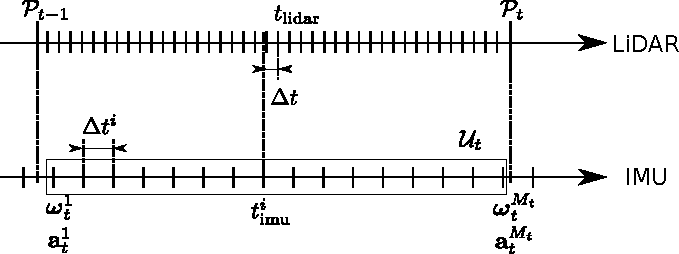
\includegraphics[width=0.6\textwidth]{../figs/time_relationships.pdf}
  \caption{Temporal relationship between LiDAR and IMU measurements.}
  \label{fig:time_relationships}
\end{figure}
















\section{IMU Preintegration}
\label{subsec:imu_preintegration}

Suppose the state ${\bf x}_{t-1}$ has been estimated up to time $t-1$, and the IMU data $\mathcal{U}_{t}$ at time $t$ is available.
In order to perform scan matching, we employ {\bf IMU preintegration} to update the rotation matrix, translation vector, and velocity vector as follows.
%
\begin{align}
  \begin{gathered}
    {}^{O}{\bf t}_{I, t} = {}^{O}{\bf t}_{I, t-1} + \sum_{i=1}^{M_{t}} {}^{O}{\bf v}_{t-1}^{j} \Delta t^{i} + \frac{1}{2} {}^{O}R_{I, t-1}^{j} \left( {\bf a}_{t}^{i} - {\bf b}_{t-1}^{a} \right) \left( \Delta t^{i} \right)^{2} + \frac{1}{2} {\bf g} \left( \Delta t^{i} \right)^{2}, \\
%
    {}^{O}R_{I, t} = {}^{O}R_{I, t-1} \prod_{i=1}^{M_{t}} \exp \left( \left( \boldsymbol \omega_{t}^{i} - {\bf b}_{t-1}^{\omega} \right)^{\wedge} \Delta t^{i} \right), \\
%
    {}^{O}{\bf v}_{t} = {}^{O}{\bf v}_{t-1} + \sum_{i=1}^{M_{t}} {}^{O}R_{I, t-1}^{j} \left( {\bf a}_{t}^{i} - {\bf b}_{t-1}^{a} \right) \Delta t^{i} + {\bf g} \Delta t^{i}, \\
  \end{gathered}
  \label{eq:discrete_imu_preintegration}
\end{align}
%
where ${\bf g}$ denotes the gravity acceleration vector, $\Delta t^{i}$ represents the time interval between the $i$-th and $(i-1)$-th IMU measurements, and ${}^{O}R_{I, t-1}^{j}$ and ${}^{O}{\bf v}_{I, t-1}^{j}$ are given as follows.
%
\begin{align}
  \begin{gathered}
    {}^{O}R_{I, t-1}^{j} = {}^{O}R_{I, t-1} \prod_{i=1}^{j} \exp \left( \left( \boldsymbol \omega_{t}^{i} - {\bf b}_{t-1}^{\omega} \right)^{\wedge} \Delta t^{i} \right), \\
%
    {}^{O}{\bf v}_{t-1}^{j} = {}^{O}{\bf v}_{t-1} + \sum_{i=1}^{j} {}^{O}R_{I, t-1}^{j} \left( {\bf a}_{t}^{i} - {\bf b}_{t-1}^{a} \right) \Delta t^{i} + {\bf g} \Delta t^{i}. \\
  \end{gathered}
\end{align}
%
In the scan matching described next, the translation vector and rotation matrix given in equation~(\ref{eq:discrete_imu_preintegration}) are used as the initial values.
















\section{LiDAR De-skewing}
\label{subsec:deskew_scan_distortion}

In general, the sampling rate of the IMU is higher than that of the LiDAR.
As a result, multiple IMU measurements can be obtained during a single LiDAR scan.
By leveraging these measurements, it is possible to compute the poses of the IMU during the LiDAR scan, as shown in equation~(\ref{eq:discrete_imu_preintegration}).
These poses can then be used to correct the positions of the LiDAR points, thereby compensating for motion-induced distortions in the scan.
This process is referred to as LiDAR de-skewing.

Before discussing de-skewing in detail, let us denote the set of $M_{t}+1$ poses obtained through IMU preintegration as $\left( {}^{O}T_{I}^{0}, \cdots, {}^{O}T_{I}^{M_{t}} \right)$, and the corresponding set of timestamps as $\left( t_{\rm imu}^{0}, \cdots, t_{\rm imu}^{M_{t}} \right)$.
Here, ${}^{O}T_{I}^{j} = \left( {}^{O}R_{I, t-1}^{j} \mid {}^{O}{\bf t}_{I, t-1}^{j} \right) \in {\rm SE}(3)$, with ${}^{O}T_{I}^{0} = {}^{O}T_{I, t-1}$ and ${}^{O}T_{I}^{M_{t}} = {}^{O}T_{I, t}$.

We assume that each LiDAR point is associated with a timestamp.
Using this timestamp, we search for the IMU interval such that $t_{\rm imu}^{i} \leq t_{\rm lidar} \leq t_{\rm imu}^{i+1} ~ \left( i = 0, \cdots, M_{t}-1 \right)$.
Suppose that a LiDAR point ${}^{L}{\bf p}$ was acquired during the interval between $t_{\rm imu}^{i}$ and $t_{\rm imu}^{i+1}$.
In this case, the corresponding IMU pose at the acquisition time of the point can be computed as follows.
%
\begin{align}
  \begin{gathered}
    \Delta t = t_{\rm lidar} - t_{\rm imu}^{i}. \\
%
    {}^{O}R_{I}^{d} = {}^{O}R_{I, t-1}^{i} \exp \left( \left( \boldsymbol \omega_{t}^{i} - {\bf b}_{t-1}^{\omega} 
\right)^{\wedge} \Delta t \right). \\
%
    {}^{O}{\bf t}_{I}^{d} = {}^{O}{\bf t}_{I, t-1}^{i} + {}^{O}{\bf v}_{t-1}^{i} \Delta t + \frac{1}{2} {}^{O}R_{I, t-1}^{i} \left( {\bf a}_{t}^{i} - {\bf b}_{t-1}^{a} \right) \Delta t^{2} + \frac{1}{2} {\bf g} \Delta t^{2}.
  \end{gathered}
\end{align}
%
Then, we define ${}^{O}T_{I}^{d} = \left( {}^{O}R_{I}^{d} \mid {}^{O}{\bf t}_{I}^{d} \right)$, and transform ${}^{L}{\bf p}$ into a point expressed in the IMU coordinate frame as follows:
%
\begin{align}
  {}^{I}{\bf p} = \left( {}^{O}T_{I}^{M_{t}} \right)^{-1} {}^{O}T_{I}^{d} {}^{I}T_{L} {}^{L}{\bf p},
\end{align}
%
where ${}^{I}T_{L}$ denotes the rigid transformation matrix between the LiDAR and the IMU, which is assumed to be known in advance through calibration.
By applying this operation to all measured points, the motion-induced distortion in the LiDAR point cloud can be corrected.
Finally, by applying $\left( {}^{O}T_{I}^{M_{t}} \right)^{-1}$, the corrected point cloud is expressed in a coordinate frame whose origin corresponds to the predicted IMU pose obtained from equation~(\ref{eq:discrete_imu_preintegration}).


















\section{Scan Matching with a Local Map}

After completing the prediction by IMU preintegration and the subsequent motion distortion correction, scan matching is performed with the local map.
For the sake of explanation, we first describe scan matching with the local map; the method for constructing the local map will be presented later in Section~\ref{subsec:local_map_building}.
As for scan matching itself, we generally apply the method described in Section~\ref{sec:scan_matching}, but in this subsection we clarify the data and coordinate frames involved.

Assume that the point cloud representing the local map, ${}^{O}\mathcal{M}$, has been constructed in the odometry frame\footnote{There are various approaches to building a local map, and in some methods the map is not explicitly constructed in the odometry frame.}.
Furthermore, after applying the distortion correction described in the previous subsection, we obtain the LiDAR point cloud in the IMU frame, denoted as ${}^{I}\mathcal{P}$.
In this case, the residual vector for a LiDAR measurement point ${}^{I}{\bf p}$ is defined as follows:
%
\begin{align}
  {\bf r} = {}^{O}{\bf q} - {}^{O}T_{I} {}^{I}{\bf p},
  \label{eq:residual_vector_lio_scan_matching}
\end{align}
%
where ${}^{O}{\bf q}$ denotes the point in ${}^{O}\mathcal{M}$ that is closest to ${}^{O}T_{I} {}^{I}{\bf p}$.
We then minimize the following cost function:
%
\begin{align}
  E \left( {}^{O}T_{I} \right) = \sum_{i=1}^{N} \rho \left( \left\| {\bf n}_{i}^{\top} {\bf r}_{i} \right\|_{2}^{2} \right),
  \label{eq:cost_function_lio_scan_matching}
\end{align}
%
where ${\bf n}$ denotes the normal vector associated with ${}^{O}{\bf q}$.














\section{State Update via Loose Coupling}

Let ${}^{O}\hat{T}_{I}$ denote the pose predicted by IMU preintegration, and let ${}^{O}T_{I}^{*}$ denote the pose obtained from scan matching.
The corresponding translation vectors and quaternions of the rotation matrices are written as ${}^{O}\hat{\bf t}_{I}$, ${}^{O}{\bf t}_{I}^{*}$, ${}^{O}\hat{\bf q}_{I}$, and ${}^{O}{\bf q}_{I}^{*}$, respectively.
Using these, the latest state is updated as follows:
%
\begin{align}
  \begin{gathered}
    {}^{O}{\bf q}_{I} = {}^{O}\hat{ {\bf q} }_{I} + \Delta t \gamma_{1} {}^{O}\hat{ {\bf q} }_{I} \left( \begin{matrix} 1 - \left| q_{w}^{d} \right| \\ {\rm sgn} \left( q_{w}^{d} \right) {\bf q}_{v}^{d} \end{matrix} \right), \\
    {\bf b}^{\omega} = \hat{ {\bf b} }^{\omega} - \Delta t \gamma_{2} q_{w}^{d} {\bf q}_{v}^{d}, \\
    {}^{O}{\bf t}_{I} = {}^{O}\hat{ {\bf t} }_{I} + \Delta t \gamma_{3} {\bf t}^{d}, \\
    {}^{O}{\bf v} = {}^{O}\hat{ {\bf v} }_{t} + \Delta t \gamma_{4} {\bf t}^{d}, \\
    {\bf b}^{a} = \hat{ {\bf b} }^{a} - \Delta t \gamma_{5} {}^{O}\hat{R}_{I}^{\top} {\bf t}^{d},
  \end{gathered}
\end{align}
%
where $\Delta t$ denotes the total integration time used in IMU preintegration, and $\gamma_{1-5}$ are arbitrary positive constants.
The relative pose is expressed as ${\bf q}^{d} = {}^{O}\hat{\bf q}_{I}^{-1} \otimes {}^{O}{\bf q}_{I}^{*}$ and ${\bf t}^{d} = {}^{O}{\bf t}_{I}^{*} - {}^{O}\hat{\bf t}_{I}$.
Furthermore, ${\bf q}^{d} = \left( q_{w}^{d} ~ \left( {\bf q}_{v}^{d} \right)^{\top} \right)^{\top}$ with ${\bf q}_{v}^{d} = \left( q_{x}^{d} ~ q_{y}^{d} ~ q_{z}^{d} \right)^{\top}$, and ${}^{O}\hat{R}_{I}$ is the rotation matrix corresponding to ${}^{O}\hat{\bf q}_{I}$.


















\section{Local Map Construction}
\label{subsec:local_map_building}

There are various ways to construct a local map; in this book, we adopt a keyframe-based approach.
Specifically, several poses estimated by the LIO are selected as keyframes, and the corresponding LiDAR point clouds are used together with those poses to construct the local map ${}^{O}\mathcal{M}$.
For keyframe detection, we employ the simplest method: a threshold is set on the amount of motion, and whenever the translational displacement or rotational displacement from the previously selected keyframe exceeds this threshold, a new keyframe is selected.

Let the set of keyframes be denoted as $\left( {}^{O}T_{I, 1}, \cdots, {}^{O}T_{I, K} \right)$, and the corresponding LiDAR point clouds as $\left( {}^{I}\mathcal{P}_{1}, \cdots, {}^{I}\mathcal{P}_{K} \right)$.
Here, $K$ represents the number of keyframes used to construct the local map.
The local map is then defined as the union of all these point clouds, each transformed into the odometry frame using their corresponding keyframe poses.
%
\begin{align}
  {}^{O}\mathcal{M} = \bigcup_{i=1}^{K} \bigcup_{{}^{I}{\bf p} \in {}^{I}\mathcal{P}_{i}} {}^{O}T_{I, i} {}^{I}{\bf p}.
\end{align}
%

The number of keyframes used may vary, but in general, the local map becomes a large point cloud.
As a result, computing normal vectors for all points would incur a very high computational cost.
Moreover, as the local map grows, it inevitably includes many points that are not actually used in scan matching.
Therefore, in our implementation, normal vectors are computed only for those points involved in the residual vector defined in equation~(\ref{eq:residual_vector_lio_scan_matching}).
Additionally, a flag is implemented to indicate whether a normal has already been computed, further reducing the computational cost associated with local map construction.














\section{Practical Considerations}

Loose-coupled LIO, compared to the tight-coupled LIO described in the next chapter, is generally easier to implement and tune.
Moreover, it delivers sufficient performance in most environments.
Therefore, it can be considered a suitable approach for those who wish to first implement LIO and understand how to fuse LiDAR and IMU measurements.
That said, tight-coupled LIO often achieves higher accuracy in practice, though at the cost of increased implementation complexity and parameter tuning difficulty.
To reiterate, loose coupling itself can provide satisfactory performance, and the choice between loose and tight coupling ultimately depends on the user's specific requirements and context.

The most computationally demanding part of LIO lies in the construction of the local map.
Reducing the map size lowers the computational cost, but also limits the spatial extent available for scan matching, which in turn increases the likelihood of drift in motion estimation.
Conversely, if the local map is too large, the computational burden grows significantly and, in the worst case, may exceed the LiDAR's measurement cycle, causing LIO to fail.

The update frequency of the local map also has a major impact on LIO accuracy.
In environments where LiDAR observations are not well suited for scan matching, increasing the update frequency of the local map helps maintain accuracy.
However, more frequent updates naturally increase computational cost.
In our implementation, local map updates are triggered when the estimated motion exceeds a fixed threshold.
Thus, increasing the update frequency results in smaller local maps, which can again make the system more prone to drift errors.
When accuracy degradation is observed, adjusting parameters related to the local map or revisiting the update policy often proves effective.
It should be noted that these issues concerning local maps also arise in tight-coupled LIO, discussed in the next chapter.



















